\documentclass{article}

\usepackage[hmargin=.65in, vmargin=.75in]{geometry}
\usepackage[citecolor=blue, colorlinks=true, linkcolor=blue, urlcolor=blue]{hyperref}
\usepackage{natbib}
\usepackage{graphicx}
\usepackage{authblk}

\title{A Standard for Exchangeable Magnetotelluric Data and Metadata}
\date{\textbf{Version 0.0.1b -- May 2020}\footnote{\noindent\textbf{\textit{Corresponding Authors:}}
		
		Jared Peacock (\url{jpeacock@usgs.gov})
		
		Andy Frassetto (\url{andy.frassetto@iris.edu})}}
\author[1]{Working Group for Data Handling and Software - PASSCAL Magnetotelluric Program}
\affil[1]{Portable Array Seismic Studies of the Continental Lithosphere, Incorporated Research Institutions for Seismology}

\newcommand{\attr}[1]{\textbf{#1}}
\renewcommand{\arraystretch}{1.35}

\begin{document}
	
\maketitle

\tableofcontents
\vspace{1cm}



%\noindent\textbf{\textit{Corresponding Authors:}}
%
%Jared Peacock (\url{jpeacock@usgs.gov})
%
%Andy Frassetto (\url{andy.frassetto@iris.edu})
\newpage

\section{Introduction}

Researchers using magnetotelluric (MT) methods lack a standardized format for storing time series data and metadata. Commercially available MT instruments produce data in formats that range from proprietary binary to ASCII, and recent datasets from the U.S. MT community have utilized institutional formats or heavily adapted formats like miniSEED. In many cases, the available metadata for these time series are incomplete and only loosely standardized, and overall these datasets are not "user friendly". This lack of resources impedes the exchange and broader use of these data beyond a small community of specialists.

The \href{https://www.iris.edu/hq/programs/passcal/magnetotelluricnstrumentation}{IRIS PASSCAL MT facility} maintains a pool of MT instruments that are freely available to U.S. Principal Investigators (PIs). Datasets collected with these instruments are subject to data sharing requirements, and an IRIS \href{https://www.iris.edu/hq/aboutris/governance/mtoft}{working group} advises the development of sustainable data formats and workflows for this facility. Following in the spirit of the standard created for \href{https://library.seg.org/doi/10.1190/geo2018-0679.1}{MT transfer function} datasets, this document outlines a new metadata standard for MT time series. This standard is a key pillar of MTH5, a new data format which we propose for the international community of MT practitioners. Further information regarding MTH5 will be available later in 2020.

The Python 3 module written for these standards are found at \url{https://github.com/kujaku11/MTarchive/tree/tables}.

\section{General Structure}

The metadata for a full MT dataset are structured to cover details from single channel time series to the full survey. For simplicity each of the different scales of an MT survey and measurements have been categorized starting from largest to smallest (Figure \ref{fig:example}. These categories are: \verb|Survey|, \verb|Station|, \verb|Run|, \verb|DataLogger|, \verb|Electric Channel|, \verb|Magnetic Channel|, and \verb|Auxiliary Channels|. Each of these are described in subsequent sections.  

\begin{figure}[htb!]
	\centering
	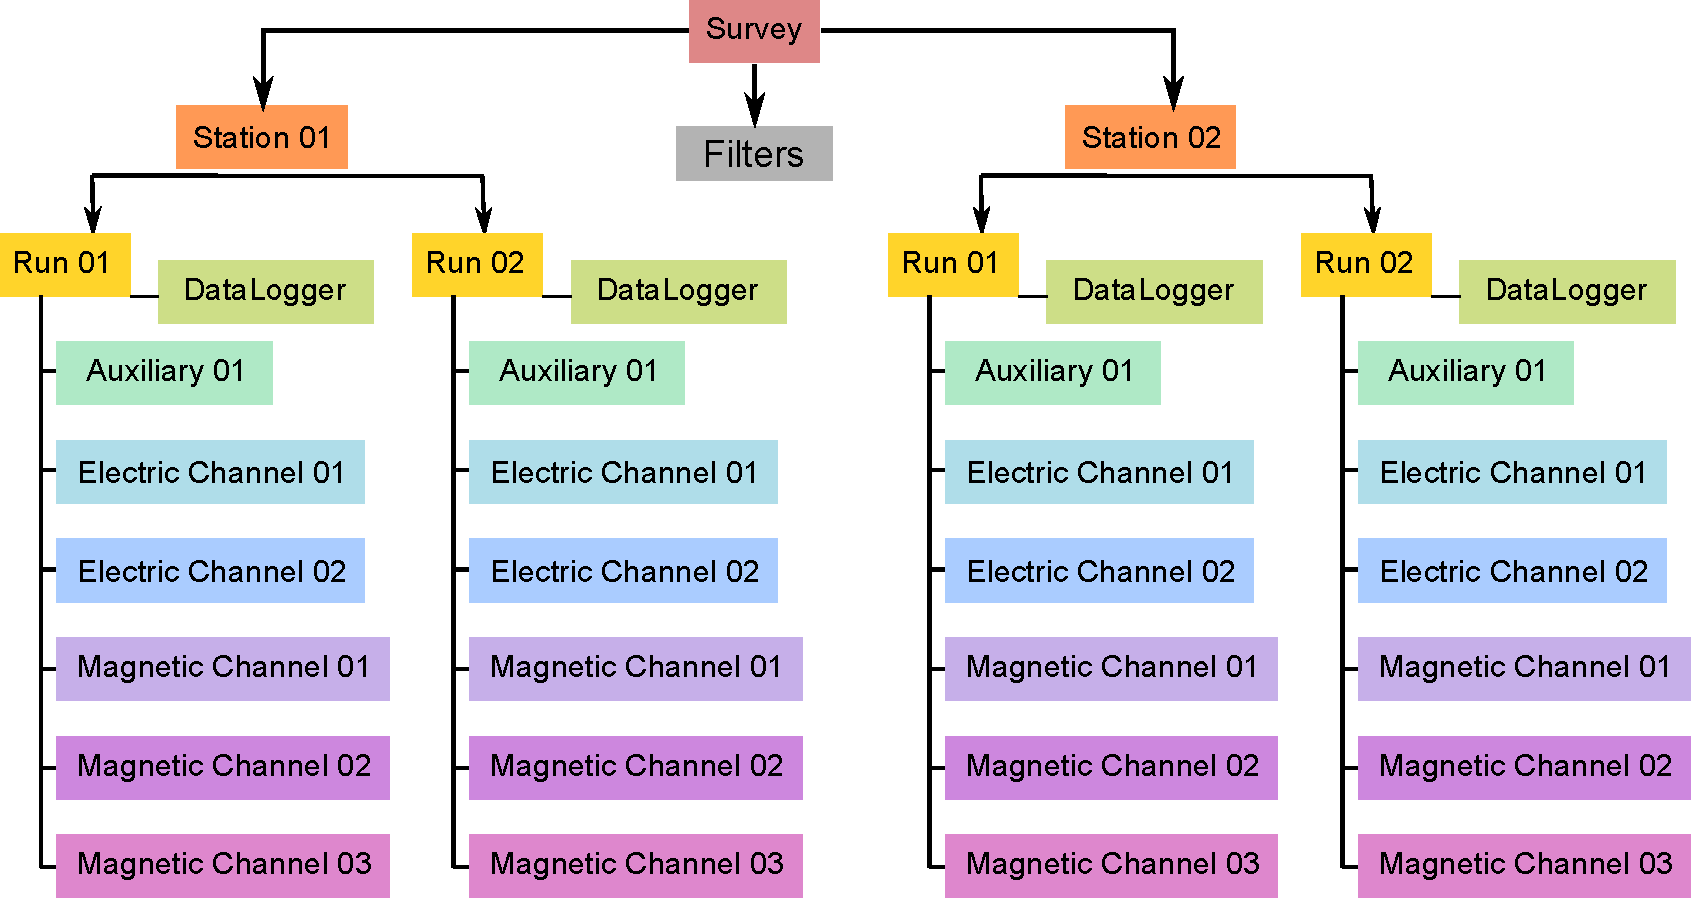
\includegraphics[height=.625\textheight]{example_mt_file_structure.pdf}
	\caption{Schematic of a MT time series file structure with appropriate metadata.}
	\label{fig:example}
\end{figure}

\subsection{Metadata Keyword Format}

The metadata key names should be self explanatory and they are structured as follows: \verb|{category}.{name}|, where:
\begin{itemize}
	\item \verb|category| refers to a metadata category that has common parameters, such as \verb|location| which will have a latitude, longitude, and elevation $\longrightarrow$ \verb|location.latitude|, \verb|location.longitude|, and \verb|location.elevation|.  These can be nested, for example \verb|positive.location.latitude|
	\item \verb|name| is the description name, where words should be separated by an underscore, e.g. \verb|data_quality|.  
\end{itemize}  

Alternatively, the metadata names can be nested under category headings as commonly done in XML or JSON formats.  See examples below for various flavors of ways to represent the metadata.      

\begin{table}[htb!]
	\caption[Data types]{Permissible values for data types}
	\centering
	\begin{tabular}{l}
		\hline
		\textbf{Data Type} \\
		\hline
		String  \\ 
		Double (float) \\
		Integer  \\ 
		Boolean  \\ \hline
	\end{tabular}
	\label{tab:types}
\end{table}

\subsection{Formatting Standards}

Specific and required formatting standards for location, time and date, and angles are defined below.

\subsubsection{Time and Date Format}

All time and dates are given as an ISO formatted date-time string in the UTC time zone.  The ISO date time format is \verb|YYYY-MM-DDThh:mm:ss.ms+00:00|.  Milliseconds can be accurate to 6 decimal places.  Dates are formatted \verb|YYYY-MM-DD|. 

\subsubsection{Location}

All latitude and longitude locations are given in decimal degrees in the well known datum   \textbf{The entire survey should use only one datum that is specified at the Survey level.}

\begin{itemize}
	\setlength\itemsep{0em}
	\item All latitude values must be $<|90|$ and all longitude values must be $<|180|$.
	\item Elevation and other distance values are given in meters.
	\item Datum should be one of the well known datums, WGS84 is preferred, but others are acceptable.
\end{itemize} 

\subsubsection{Angles}

All angles of orientation are given in degrees.  Orientation of dipoles and magnetometers should be given in geographic coordinates where angles are assumed to be clockwise positive from Geographic North = 0.  If a station was collected not in geographic coordinates this needs to be specified in \verb|station.orientation.option|.   

\subsection{Units}
Units should all be from the metric system.  Abbreviations and full names are acceptable, for example \verb|mV| and \verb|millivolts|.  Below are a summary of common acceptable units:


\begin{table}[htb!]
	\centering
	\caption[Acceptable units]{Acceptable units}
	\begin{tabular}{|l|c|c|}
		\hline
		\textbf{Measurement Type} & \textbf{Unit Long Name}  & \textbf{Unit Short Name} \\ \hline
		Angles & degrees & deg \\ \hline
		
		Distance &  meters & m \\ \hline
		Latitude/Longitude & decimal degrees & deg \\ \hline
		Resistance & Ohms  &  Ohms \\ \hline
		Resistivity & Ohm-meters & Ohm-m, Ohmm \\ \hline
		Temperature & Celsius & C \\ \hline
		Time & seconds & s \\ \hline
		Voltage & Volts & V \\ \hline
		
		
	\end{tabular}
	\label{tab:units}
\end{table}

\subsection{String Formats}

Any list should be comma separated.

\begin{table}[htb!]
	\centering
	\caption[Acceptable String Formats]{Acceptable String Formats}
	\begin{tabular}{|l|p{3.5in}|c|}
		\hline
		\textbf{Style} & \textbf{Description}  & \textbf{Example} \\ \hline
		free form & an unregulated string that can contain \{a-z, A-Z, 0-9\} and special characters & This is free form! \\ \hline
		
		alpha numeric & a string that contains no spaces and only characters \{a-z, A-Z, 0-9, -, /, \_\} & WGS84 or GEOMAG-USGS \\ \hline
		controlled vocabulary & Only certain names or words are allowed &  station.orientation.option = geographic \\ \hline
		url & a full URL that a user could put into a web browser  &  \url{https://www.passcal.nmt.edu/} \\ \hline
		date & ISO formatted date YYYY-MM-DD in UTC & 2020-02-02 \\ \hline
		date time & ISO formatted date time YYYY-MM-DDThh:mm:ss.ms+00:00 in UTC & 2020-02-02T12:20:45.123456+00:00 \\ \hline
		Temperature & Celsius & C \\ \hline
		Time &  seconds & s \\ \hline
		Voltage & Volts & V \\ \hline
		
		
	\end{tabular}
	\label{tab:values}
\end{table}

\clearpage
\newpage
\section{Survey}

A survey describes an entire dataset that covers a specific time span and region. This may include multiple PIs in multiple data collection episodes but should be confined to a specific experiment. The \verb|Survey| metadata category describes the general parameters of the survey.

\begin{table}
	\centering
	\caption[Attributes for Survey]{Attributes for Survey category}
	\begin{tabular}{|l|p{2.75in}|l|c|p{.95in}|}
		\hline
		\textbf{Metadata Key} & \textbf{Description} & \textbf{Type} & \textbf{Required}  & \textbf{Style}  \\ \hline
		acquired\_by.author\ & principal investigator(s) responsible for survey & string & true & free form  \\ \hline
		acquired\_by.comments\ & comments about who acquired the data, could include the various groups or contractors & string & true & free form \\ \hline
		archive\_id & alphanumeric name for the project e.g USGS-GEOMAG & string & true & alpha numeric  \\ \hline
		archive\_network & network code given by PASSCAL/IRIS/FDSN & string & true & alpha numeric  \\ \hline
		citation\_data\_set.doi & citation dataset doi number & string & true & url  \\ \hline
		citation\_journal.doi & citation journal doi & string & false & url  \\ \hline
		comments\ & comments about survey that are not in the summary & string & false & free form \\ \hline
		country\ & country/countries survey located in, if multiple they should be comma separated & string & false & free form \\ \hline
		datum\ & datum of latitude and longitude coordinates, should be a well-known datum [ WGS84 ] and will be the reference datum for all location & string & true & alpha numeric \\ \hline
		geographic\_name\ & geographic location(s) of survey in general terms & string & true & free form \\ \hline
		name\ & descriptive name of the survey & string & true & free form \\ \hline
		northwest\_corner.latitude\ & location of northwest corner of survey [ degrees ] & float & true & number \\ \hline
		northwest\_corner.longitude\ & location of northwest corner of survey [ degrees] & float & true & number \\ \hline
		project & alphanumeric name for the project e.g USGS-GEOMAG & string & true & alpha numeric  \\ \hline
		project\_lead.email & email address of the project lead & string & true & email  \\ \hline
		project\_lead.name & name of the project lead & string & true & free form  \\ \hline
		project\_lead.organization & name of the organization for the project lead & string & true & free form  \\ \hline
		release\_status\ & defined status of how the data can be used. Options are [ Unrestricted Release $|$ Paper Citation Required $|$ Academic Use Only $|$ Conditions Apply ] & string & true & controlled vocabulary \\ \hline
		southeast\_corner.latitude\ & location of southeast corner of survey [degrees] & float & true & number \\ \hline
		southeast\_corner.longitude\ & location of southeast corner of survey [degrees] & float & true & number \\ \hline
		summary\ & summary paragraph of survey including the purpose, difficulties, data quality, summary of outcomes if the data have been processed and modeled & string & true & free form \\ \hline
		time\_period.end\_date\ & end date of survey in UTC & string & true & date  \\ \hline
		time\_period.start\_date\ & start date of survey in UTC & string & true & date \\ \hline
	
	\end{tabular}
	\label{tab:survey}
\end{table} 

\newpage
\subsection{Example Survey XML String}

\begin{verbatim}
<?xml version="1.0" ?>
<survey>
    <acquired_by>
        <author>None</author>
        <comments>None</comments>
    </acquired_by>
    <archive_id>None</archive_id>
    <archive_network>None</archive_network>
    <citation_dataset>
        <doi>None</doi>
    </citation_dataset>
    <citation_journal>
        <doi>None</doi>
    </citation_journal>
    <comments>None</comments>
    <country>None</country>
    <datum>None</datum>
    <geographic_name>None</geographic_name>
    <name>None</name>
    <northwest_corner>
        <latitude type="float" units="decimal degrees">None</latitude>
        <longitude type="float" units="decimal degrees">None</longitude>
    </northwest_corner>
    <project>None</project>
    <project_lead>
        <email>None</email>
        <organization>None</organization>
        <author>None</author>
    </project_lead>
    <release_status>None</release_status>
    <southeast_corner>
        <latitude type="float" units="decimal degrees">None</latitude>
        <longitude type="float" units="decimal degrees">None</longitude>
    </southeast_corner>
    <summary>None</summary>
    <time_period>
        <end_date>1980-01-01</end_date>
        <start_date>1980-01-01</start_date>
    </time_period>
</survey>
\end{verbatim}

\newpage
\section{Station}

A station encompasses a single site where data are collected. If the location changes during a run, then a new station should be created. If the sensors, cables, data logger, battery are replaced during a run but the station remains stations, then this can be recorded in the \verb|Run| metadata but does not require a new station entry.

\begin{table}[htb!]
    \caption[Attributes for Station]{Attributes for Station category}
    \begin{tabular}{|l|p{3in}|l|l|}
        \hline
        \textbf{Metadata Key} & \textbf{Description} & \textbf{Type} & \textbf{Required} \\ \hline
        archive\_id\ & 5 char name {A-Z; 1-9} for station & string & true \\ \hline
        id\ & general name for station & string & true \\ \hline
        geographic\_name\ & closest geographic reference name to station  & string & true \\ \hline
        location.latitude\ & longitude location [ degrees (hh.mmss) ] & float & true \\ \hline
        location.longitude\ & latitude location [ degrees (hh.mmss) ] & float & true \\ \hline
        location.elevation\ & elevation [ m ] & float & true \\ \hline
        location.datum\ & datum for lat, lon location should be a well known datum and same as the survey datum & string & true \\ \hline
        location.declination.value\ & declination value & float & true \\ \hline
        location.declination.epoch\ & declination epoch & string & true \\ \hline
        location.declination.model\ & declination model & string & true \\ \hline
        comments\ & any comments about station & string & false \\ \hline 
        time\_period.start\ & start time and date of data logging [ISO UTC ] & string & true \\ \hline
        time\_period.end\ & stop time and date of data logging  [ ISO UTC ] & string & true \\ \hline
        num\_channels\ & number of channels recording needs to be the same number as entries in channels\_recorded & int & true \\ \hline
        channels\_recorded\ & list of channels recorded [EX, EY, HX, HY, HZ $|$ ...], needs to be same length as num\_channels & string & true \\ \hline
        data\_type\ & type of data collected [ BB $|$ LP $|$ AMT $|$ Combo $|$ ...] & string & true \\ \hline
        orientation.option & orientation coordinate system [ geographic $|$ channel-measurement specific $|$ ...] & string & true \\ \hline
        orientation.method & [ compass $|$ differential GPS $|$ gyroscope $|$...] & string & false \\ \hline
%        acquired\_by.author & person(s) operating station & string & true \\ \hline
%        acquired\_by.email & email of lead station operator & string & true \\ \hline
        provenance.creation\_time & creation time of time series data for storing & string & true \\ \hline
        provenance.software.name\ & name of software used to store time series & string & true \\ \hline
        provenance.software.version\ & version of software used to store time series & string & true \\ \hline
        provenance.submitter.author\ & name of person or group submitting archive data & string & true \\ \hline
        provenance.submitter.organization\ & name of organization or institution submitting archive data & string & true \\ \hline
        provenance.submitter.url\ & url of group submitting archive data & string & true \\ \hline
        provenance.submitter.email\ & email of person or group submitting archive data & string & true  \\ \hline
        provenance.comments\ & any comments on the history of the data & string & false \\ \hline
        provenance.log\ & log of any changes made to time series data & string & false \\ \hline
    \end{tabular}
\label{tab:station01}
\end{table}    
   
\newpage
\subsection{Example Station JSON String}

\begin{verbatim}
{
    "station": {
        "archive_id": "test sta_code",
        "channels_recorded": "[ex, ey, hx, hy, hz]",
        "comments": "comments test",
        "data_type": "MT",
        "geographic_name": "Paris, TX",
        "id": "test name",
        "location.datum": "WGS84",
        "location.declination.epoch": "MTM01",
        "location.declination.model": "MTM01",
        "location.declination.value": -12.3,
        "location.elevation": 1230.0,
        "location.latitude": 40.019,
        "location.longitude": -117.89,
        "num_channels": 5,
        "orientation.method": "compass",
        "orientation.option": "geographic north",
        "provenance.comments": "goats",
        "provenance.creation_time": "2010-04-01T10:10:10+00:00",
        "provenance.log": "EY flipped",
        "provenance.software.author": "Peacock",
        "provenance.software.name": "mth5",
        "provenance.software.version": "1.0.1",
        "provenance.submitter.author": "submitter name",
        "provenance.submitter.email": "mt@em.edi",
        "provenance.submitter.organization": "mt inc",
        "provenance.submitter.url": "mt.edi",
        "time_period.end": "2010-01-04T07:40:30+00:00",
        "time_period.start": "2010-01-01T12:30:20+00:00"
    }
}
\end{verbatim}

\newpage
\section{Run}

A run represents data collected at a single station with a single sampling rate. If the dipole length or other such station parameters are changed between runs, this would require adding a new run.  If the station is relocated then a new station should be created.  If a run has channels that drop out the start and end period will be the minimum time and maximum time for all channels recorded.

\begin{table}[htb!]
    \caption[Attributes for Run]{Attributes for Run category}
    \begin{tabular}{|l|p{3.2in}|l|l|}
        \hline
        \textbf{Metadata Key} & \textbf{Description} & \textbf{Type} & \textbf{Required} \\ \hline
        id\ & run ID & string & true \\ \hline
        comments\ & comments on run, commonly station name with {0-9}{0-9} or {a-z}, mt01a or mt01\_01 & string & false \\ \hline
        time\_period.start\ & start date and time of data logging [ ISO UTC ], should be the minimum time between all channels recorded & string & true \\ \hline
        time\_period.end\ & stop date and time of data logging [ ISO UTC ], should be the maximum time between all channels recorded & string & true \\ \hline
        sampling\_rate\ & sampling rate of run (samples per second) & float & true \\ \hline
%        num\_channels\ & number of channels recorded & int & true \\ \hline
        channels\_recorded\ & list of channels recorded as components [ [EX, EY, HX, HY] $|$ ...] & string & true \\ \hline
        data\_type \ & type of data collected [ BB $|$ LP $|$ AMT $|$ Combo $|$ ...] & string & true \\ \hline
        acquired\_by.author\ & person(s) responsible for run this can be different from the PI's listed at he survey level & string & true \\ \hline
        acquired\_by.email\ & email of lead run operator & string & false \\ \hline
        provenance.comments\ & any comments on the history of the data for the run & string & false \\ \hline
        provenance.log\ & log of any changes made to time series data & string & false \\ \hline
        data\_logger.manufacturer\ & data logger manufacturer name & string & true \\ \hline
        data\_logger.model\ & data logger model name & string & true \\ \hline
        data\_logger.serial\ & data logger serial number & string & true \\ \hline
        data\_logger.comments\ & comments about data logger & string & true \\ \hline
        data\_logger.timing\_system.type\ & type of timing system [GPS $|$ internal $|$ ... ] & string & true \\ \hline
        data\_logger.timing\_system.drift\ & any drift in internal clock [ seconds ] & float & true \\ \hline
        data\_logger.timing\_system.uncertainty\ & uncertainty associated with internal clock [seconds] & float & true \\ \hline
        data\_logger.timing\_system.comments\ & comments on timing system & string & false \\ \hline
        data\_logger.firmware.version\ & firmware version & string & true \\ \hline
        data\_logger.firmware.date\ & date on firmware & string & true \\ \hline
        data\_logger.firmware.author\ & author of firmware & string & false \\ \hline
%        n\_channels\ & number of channels & int & true \\ \hline
%        n\_channels\_used\ & number of channels used & int & true \\ \hline
        data\_logger.power\_source.type\ & power source type [ Pb-acid battery $|$ solar panel $|$ Li battery $|$ ...] & string & true \\ \hline
        data\_logger.power\_source.id\ & power source id & string & false \\ \hline
        data\_logger.power\_source.voltage.start\ & starting voltage of power source & float & true \\ \hline
        data\_logger.power\_source.volage.end\ & ending voltage of power source & float & true \\ \hline
        data\_logger.power\_source.comments\ & comments on power source & string & false \\ \hline
    \end{tabular}
    \label{tab:run}
\end{table}

\subsection{Example Run XML String}

\begin{verbatim}
<run>
    <acquired_by>
        <author>T. Lurric</author>
        <email>mt@mt.org</email>
    </acquired_by>
    <channels_recorded>[EX, EY, HX, HY, HZ, temperature]</channels_recorded>
    <comments>None</comments>
    <data_logger>
        <power_source>
            <voltage>
                <start type="float" units="volts">14</start>
                <end type="float" units="volts">12</end>
            </voltage>
            <type>pb-acid</type>
            <id>10</id>
            <comments>solar panel</comments>
        </power_source>
        <id>mt01</id>
        <manufacturer>MT r' Us</manufacturer>
        <type>broadband</type>
        <timing_system>
            <type>GPS</type>
            <drift type="float" units="seconds">0.00001</drift>
            <uncertainty type="float" units="seconds">0.00001</uncertainty>
            <notes>None</notes>
        </timing_system>
        <firmware>
            <author>MT r' Us</author>
            <version>12.15.a</version>
            <name>FGDMT</name>
        </firmware>
    </data_logger>
    <data_type>MT</data_type>
    <id>mt01a</id>
    <provenance>
        <comments>None</comments>
        <log>None</log>
    </provenance>
    <sampling_rate type="float" units="samples per second">256.0</sampling_rate>
    <time_period>
        <start>1980-01-01T00:00:00+00:00</start>
        <end>1980-01-01T00:00:00+00:00</end>
    </time_period>
</run>
\end{verbatim}

%\newpage
%\section{Data Logger}
%
%Data logger is a the digital acquisition system used to collect time series data at a single station for a single run.  \verb|DataLogger| metadata includes the type of data logger, timing system, firmware, number of channels, calibrations, and power source.
%
%\begin{table}[htb!]
%    \caption[Attributes for DataLogger]{Attributes for DataLogger category}
%    \begin{tabular}{|l|p{3in}|l|l|}
%        \hline
%        \textbf{Metadata Key} & \textbf{Description} & \textbf{Type} & \textbf{Required} \\ \hline
%        manufacturer\ & manufacturer name & string & true \\ \hline
%        model\ & model name & string & true \\ \hline
%        serial\ & serial number & string & true \\ \hline
%        comments\ & comments about data logger & string & true \\ \hline
%        timing\_system.type\ & type of timing system [GPS $|$ internal $|$ ... ] & string & true \\ \hline
%        timing\_system.drift\ & any drift in internal clock [ seconds ] & float & true \\ \hline
%        timing\_system.uncertainty\ & uncertainty associated with internal clock [seconds] & float & true \\ \hline
%        timing\_system.comments\ & comments on timing system & string & false \\ \hline
%        firmware.version\ & firmware version & string & true \\ \hline
%        firmware.date\ & date on firmware & string & true \\ \hline
%        firmware.author\ & author of firmware & string & false \\ \hline
%        n\_channels\ & number of channels & int & true \\ \hline
%        n\_channels\_used\ & number of channels used & int & true \\ \hline
%        power\_source.type\ & power source type [ Pb-acid battery $|$ solar panel $|$ Li battery $|$ ...] & string & true \\ \hline
%        power\_source.id\ & power source id & string & false \\ \hline
%        power\_source.voltage.start\ & starting voltage of power source & float & true \\ \hline
%        power\_source.volage.end\ & ending voltage of power source & float & true \\ \hline
%        power\_source.comments\ & comments on power source & string & false \\ \hline
%    \end{tabular}
%    \label{tab:datalogger}
%\end{table}    
%
%\newpage
%\subsection{Example DataLogger JSON String}
%
%\begin{verbatim}
%{
% "manufacturer": "MT `r Us",
% "model": "Broadband 2000",
% "serial": "0128947850230",
% "comments": "Intern dropped the data logger on a shovel.",
% "timingystem.type": "GPS",
% "timingystem.drift": 0,
% "timingystem.uncertainty": 0.0016,
% "timingystem.comments": "only works when sky is clear",
% "firmware.version": "1.0",
% "firmware.date": "2020-01-01",
% "firmware.author": "R. Phase",
% "n_channels": 5,
% "n_channels_used": 4,
% "powersource.id": "battery 10"
% "powersource.type": "solar panel and battery",
% "powersource.voltage.start": 13.1,
% "powersource.voltage.end": 12.0,
% "powersource.comments": "Overcast all day reduced recharging"
%}
%\end{verbatim}

\newpage
\section{Electric Channel}

Electric channel refers to a dipole measurement of the electric field for a single station for a single run.   
 
\begin{table}[htb!]
    \caption[Attributes for Electric Channel]{Attributes for Electric category}
    \begin{tabular}{|l|p{3in}|l|l|}
        \hline
        \textbf{Metadata Key} & \textbf{Description} & \textbf{Type} & \textbf{Required} \\ \hline
        dipole\_length\ & length of dipole [ m ] & float & true \\ \hline
        channel\_number\ & channel number [ 1 $|$ 2 $|$ 3 $|$ 4 $|$ 5 $|$ 6 $|$...] & int & true \\ \hline
        component\ & [ Ex $|$ Ey $|$ Ez ] & string  & true \\ \hline
        azimuth\ & azimuth of dipole N = 0,  E = 90 [ degrees ] & float & true \\ \hline
        time\_period.start\ & start date and time of data logging [ ISO UTC ] & string & true \\ \hline
        time\_period.end\ & stop date and time of data logging [ ISO UTC ] & string & true \\ \hline
        positive.id\ & sensor id number & string & true \\ \hline
        positive.latitude\ & positive sensor location latitude [ degrees (hh.mmss) ] & float & false \\ \hline
        positive.longitude\ & positive sensor location longitude [ degrees (hh.mmss) ] & float & false \\ \hline
        positive.elevation\ & positive sensor location elevation [ m ] & float & false \\ \hline
        positive.datum\ & positive datum for location [ WGS84 ] & string & false \\ \hline
        positive.type\ & type of electric sensor [ Ag-AgCl $|$ Pb-PbCl $|$ ...] & string & true \\ \hline
        positive.manufacturer\ & electric sensor manufacturer & string & true \\ \hline
        positive.comments\ & comments on electric sensor & string & false \\ \hline
        negative.id\ & sensor id number & string & true \\ \hline
        negative.longitude\ & negative sensor location latitude [ degrees (hh.mmss) ] & float & false \\ \hline
        negative.latitude\ & negative sensor location longitude [ degrees (hh.mmss) ] & float & false \\ \hline
        negative.elevation\ & negative sensor location elevation [ m ] & float & false \\ \hline
        negative.datum\ & negative datum for location [ WGS84 ] & string & false \\ \hline
        negative.type\ & type of electric sensor [ Ag-AgCl $|$ Pb-PbCl $|$ ...] & string & true \\ \hline
        negative.manufacturer\ & electric sensor manufacturer & string & true \\ \hline
        negative.comments\ & comments on electric sensor & string & false \\ \hline
        contact\_resistance\_1.start\ & contact resistance at beginning of measurement, positive polarity [ Ohm ]" & float & false \\ \hline
        contact\_resistance\_2.start\ & contact resistance at beginning of measurement, negative polarity [ Ohm ] & float & false \\ \hline
        contact\_resistance\_1.end\ & contact resistance at end of measurement, positive polarity [ Ohm ] & float & false \\ \hline
        contact\_resistance\_2.end\ & contact resistance at end of measurement, negative polarity [ Ohm ] & float & false \\ \hline
        ac.start\ & AC at start of measurement [ V ] & float & false \\ \hline
        ac.end\ & AC at end of measurement [ V ] & float & false \\ \hline
        dc.start\ & DC at start of measurement [ V ] & float & false \\ \hline
        dc.end\ & DC at end of measurement [ V ] & float & false \\ \hline
        
    \end{tabular}
    \label{tab:electric01}
\end{table}    

\newpage
\begin{table}[htb!]
    \caption[Attributes for Electric Channel cont`d]{Attributes for Electric category continued}
    \begin{tabular}{|l|p{3in}|l|l|}
        \hline
        \textbf{Metadata Key} & \textbf{Description} & \textbf{Type} & \textbf{Required} \\ \hline
        units\ & units of electric field data [ counts $|$ mV/km $|$ ... ] & string & true \\ \hline
        sample\_rate\ & sample rate of electric channel (samples.second) & float & true \\ \hline
        comments\ & comments about electric field measurement & string &  false \\ \hline
        data\_quality.rating\ & data quality rating based on some sort of statistic & integer & false \\ \hline
        data\_quality.warning\_comments\ & any warnings about data quality & string & false \\ \hline
        data\_quality.warning\_flags\ & a value flagging bad data  & float &  integer \\ \hline
        data\_quality.author\ & person who did QA/QC on data & string &  false \\ \hline
        filter.name\ & filter name in filter table, can be a list. Needs to be ordered in which filters were applied & string &  false \\ \hline
        filter.comments\ & any comments on the filtering & string &  false \\ \hline
        filter.applied\_b & have filters been applied [ True $|$ False ] & string & true \\ \hline
        \end{tabular}
        \label{tab:electric02}
\end{table}    

\newpage
\subsection{Example Electric Channel JSON String}

\begin{verbatim}
{
 "dipole_length": 59.7,
 "channel_number": "1",
 "component": "EX",
 "azimuth": 0,
 "time_period.start": 2020-01-02T12:30:15+00:00,
 "time_period.end": 2020-01-05T16:20:15+00:00,
 "positive.id": "101",
 "positive.latitude": 35.5578,
 "positive.longitude": -117.38754,
 "positive.elevation": 103.4,
 "positive.datum": "WGS84",
 "positive.type": "Ag-AgCl",
 "positive.manufacturer": "Zaps",
 "positive.comments": "Sitting on the shelf since last year",
 "negative.id": "102",
 "negative.latitude": 35.5588,
 "negative.longitude": -117.38754,
 "negative.elevation": 105.8,
 "negative.datum": "WGS84",
 "negative.type": "Ag-AgCl"
 "negative.manufacturer": "Zaps",
 "negative.comments": "Sitting on the shelf since last year",
 "contact_resistance_1.start": 1200.0,
 "contact_resistance_2.start": 1210.0,
 "contact_resistance_1.end": 1205.0,
 "contact_resistance_2.end": 1205.0,
 "ac.start": 0.03,
 "ac.end": 0.04,
 "dc.start": 0.001,
 "dc.end": 0.002,
 "units": "counts",
 "sample_rate": 256,
 "comments": "cables chewed on 2020-01-07",
 "data_quality.rating": 3,
 "data_quality.warning_comments": "cables chewed 2020-01-07",
 "data_quality.warning_flags": "Nan",
 "data_quality.author": "Q. Sea",
 "filter.name": "[counts2mv, datalogger024]",
 "filter.comments": "comments on filters applied",
 "filter.applied_b": "true"
}
\end{verbatim}

\newpage
\section{Magnetic Channel}

A magnetic channel is a recording of one component of the magnetic field at a single station for a single run.

\begin{table}[htb!]
    \caption[Attributes for Magnetic Channel]{Attributes for Magnetic category}
    \begin{tabular}{|l|p{3in}|l|l|}
        \hline
        \textbf{Metadata Key} & \textbf{Description} & \textbf{Type} & \textbf{Required} \\ \hline
        sensor.type\ & type of magnetic sensor [ Induction Coil $|$ flux gate $|$ ...] & string & true \\ \hline
        sensor.manufacturer\ & magnetic sensor manufacturer & string &  true \\ \hline
        sensor.comments\ & comments on sensor & string & true \\ \hline
        sensor.id\ & sensor id number & string &  true \\ \hline
        channel\_number\ & channel number [ 1 $|$ 2 $|$ 3 $|$ 4 $|$ 5 $|$ 6 $|$...] & int &  true \\ \hline
        component\ & [ Hx $|$ Hy $|$ Hz ] & string  &  true \\ \hline
        azimuth\ & azimuth in \verb|station\_coordinates| [ degrees ]& float & true \\ \hline
        time\_period.start\ & start date and time of data logging [ ISO UTC ] & string & true \\ \hline
        time\_period.end\ & stop date and time of data logging [ ISO UTC ] & string & true \\ \hline
        location.longitude\ & sensor longitude degrees & float & true \\ \hline
        location.latitude\ & sensor latitude in degrees & float &  true \\ \hline
        location.elevation\ & sensor elevation in meters & float &  true \\ \hline
        location.datum\ & datum for location [ WGS84 $|$ ... ] & string &  true\\ \hline
        units\ & units of magnetic field data [ counts $|$ mV $|$ ... ] & string &  true \\ \hline
        sample\_rate\ & sample rate of magnetic channel (samples.second) & float &  true \\ \hline
        h\_field\_min.start\ & minimum h-field value at beginning of measurement & float &  false \\ \hline
        h\_field\_max.start\ & maximum h-field value at beginning of measurement & float &  false\\ \hline
        h\_field\_min.end\ & minimum h-field value at end of measurement & float &  false\\ \hline
        h\_field\_max.end\ & maximum h-field value at end of measurement & float &  false\\ \hline
        h\_field.units\ & units of h-field measurement [ nT $|$ ...] & string &   false \\ \hline
        comments\ & comments on magnetic field measurments & string &  false \\ \hline
        data\_quality.rating\ & data quality rating based on some sort of statistic & integer &  false \\ \hline
        data\_quality.warning\_comments\ & any warnings about data quality & string &   false \\ \hline
        data\_quality.warning\_flags\ & a value flagging bad data  & integer &  false \\ \hline
        data\_quality.author\ & person who did QC.QA on data & string &   false \\ \hline
        filter.name\ & filter name in filter table, can be a list. Needs to be ordered in which filters were applied & string &  false \\ \hline
        filter.comments\ & any comments on the filtering & string &  false \\ \hline
        filter.applied\_b & have filters been applied [ True $|$ False ] & string & true \\ \hline
        \end{tabular}
    \label{tab:magnetic}
\end{table}

\newpage
\subsection{Example Magnetic Channel JSON String}

\begin{verbatim}
{
 "sensor.type": "Induction Coil",
 "sensor.manufacturer": "MT `r Us",
 "sensor.comments": "new coil",
 "sensor.id": "2149",
 "channel_number": 5,
 "component": "HZ",
 "azimuth": 90,
 "time_period.start": 2020-01-02T12:30:15+00:00,
 "time_period.end": 2020-01-05T16:20:15+00:00,
 "location.longitude": -117.0,
 "location.latitude": 45.0,
 "location.elevation": 107.4,
 "location.datum": "WGS84",
 "units": "counts",
 "sample_rate": 256,
 "h_field_min.start": -10,
 "h_field_max.start": 10,
 "h_field_min.end": -9,
 "h_field_max.end": 9,
 "h_field.units": "nT",
 "comments": "not buried all the way ",
 "data_quality.rating": 4,
 "data_quality.warning_comments": "windy during the day",
 "data_quality.warning_flags": 0,
 "data_quality.author": "Q. Sea",
 "filter.name": "[counts2mv, datalogger024, coil2149]",
 "filter.comments": "Calibrated 2018-01-01",
 "filter.applied_b": "[true, false, false]"
}
\end{verbatim}

\newpage
\section{Filters}

Filters is a table that holds information on any filters that need to be applied to get physical units, and filters that were applied to the data to analyze the signal.  This includes calibrations, notch filters, conversion of counts to units, etc. The actual filter will be an array of numbers contained within an array named \verb|name| and formatted according to \verb|type|. The preferred format for a filter is a look-up table which internally can be converted to other formats. 

It is important to note that filters will be identified by name and must be consistent throughout the file. Names should be descriptive and self evident. Examples:
\begin{itemize}
    \item \verb|coil_2284| $\longrightarrow$ induction coil number 2284
    \item \verb|counts2mv| $\longrightarrow$ conversion from counts to mV
    \item \verb|e_gain| $\longrightarrow$ electric field gain 
    \item \verb|datalogger_024| $\longrightarrow$ data logger number 24 response
    \item \verb|notch_60hz| $\longrightarrow$ notch filter for 60 Hz and harmonics
    \item \verb|lowpass_10hz| $\longrightarrow$ low pass filter below 10 Hz
\end{itemize}

In each channel there are keys to identify filters that can or have been applied to the data to get an appropriate signal.  This can be a list of filter names or a single filter name.  An \verb|applied_b| key also exists for the user to input whether that filter has been applied.  Can be a single Boolean \verb|true| if all filters have been applied, \verb|false| if none of the filters have been applied.  Or can be a list the same length and the filter name list identifying if the filter has been applied.  \verb|name: "[counts2mv, notch60hz, e_gain]"| and \verb|applied_b: "[true, false, true]"|. 

\begin{table}[htb!]
    \caption[Attributes for Filter]{Attributes for Filters}
    \begin{tabular}{|l|p{3.5in}|l|l|}
        \hline
        \textbf{Metadata Key} & \textbf{Description} & \textbf{Type} & \textbf{Required} \\ \hline
        type\ & type of filter [look up $|$ poles-zeros $|$ converter $|$ FIR $|$ ...]& string &  true \\ \hline
        name\ & unique name for the filter such that it is easy to query & string & true \\ \hline
        units\_in\ & units of data going in [ counts $|$ mV/km $|$ ... ] & string & true \\ \hline
        units\_out\ & units of data coming out [ counts $|$ mV/km $|$ ... ] & string & true \\ \hline
        calibration\_date\ & date of calibration & string &  true \\ \hline
        comments\ & any comments on the filtering & string &  false \\ \hline
    \end{tabular}
    \label{tab:filter}
\end{table}

\subsection{Example Filter JSON String} 

\begin{verbatim}
{
 "type": "look up",
 "name": "coil_8897",
 "units_in": "mV",
 "units_out": "mV",
 "calibrationate": "2015-07-01",
 "comments": "interpolated from poles and zeros"
}
\end{verbatim}

\newpage

\section{Auxiliary Channels}

Auxiliary channels include state of health channels, temperature, etc.  

\begin{table}[htb!]
    \caption[Attributes for Auxiliary Channel]{Attributes for Auxiliary category}
    \begin{tabular}{|l|p{3in}|l|l|}
        \hline
        \textbf{Metadata Key} & \textbf{Description} & \textbf{Type} & \textbf{Required} \\ \hline
        type\ & type of data recorded [ temperature $|$ GPS $|$ ...] & string & true \\ \hline
        units\ & units of magnetic field data [ counts $|$ mV $|$ ... ] & string &  true \\ \hline
        channel\_num\ & channel number [ 1 $|$ 2 $|$ 3 $|$ 4 $|$ 5 $|$ 6 $|$...] & int &  true \\ \hline
        component\ & channel number [ `None' $|$ ... ] & string &  true \\ \hline
        sample\_rate\ & sample rate (samples.second) & float &  true \\ \hline
        comments\ & any comments on the auxillary channel & string &  false \\ \hline
        data\_quality.rating\ & data quality rating based on some sort of statistic & integer &  false \\ \hline
        data\_quality.warning\_comments\ & any warnings about data quality & string &   false \\ \hline
        data\_quality.warning\_flags\ & a value flagging bad data  & integer &  false \\ \hline
        data\_quality.author\ & person who did QC.QA on data & string &   false \\ \hline
        filter.name\ & filter name in filter table, can be a list. Needs to be ordered in which filters were applied & string &  false \\ \hline
        filter.comments\ & any comments on the filtering & string &  false \\ \hline
        filter.applied\_b & have filters been applied [ True $|$ False ] & string & true \\ \hline
    \end{tabular}
    \label{tab:aux}
\end{table}

\subsection{Example Auxiliary JSON String} 

\begin{verbatim}
{
    "auxiliary": {
         "azimuth": 0.0,
         "channel_number": 1,
         "comments": null,
         "component": "temperature",
         "data_quality.author": "mt",
         "data_quality.rating": 5,
         "data_quality.warning_comments": null,
         "data_quality.warning_flags": "0",
         "filter.applied": [false],
         "filter.comments": null,
         "filter.name": ["counts2mv"],
         "location.datum": "WGS84",
         "location.elevation": 1200.3,
         "location.latitude": 40.12,
         "location.longitude": -115.767,
         "sample_rate": 256.0,
         "time_period.end": "2010-01-04T07:40:30+00:00",
         "time_period.start": "2010-01-01T12:30:20+00:00",
         "type": "auxiliary",
         "units": "celsius"
    }
}
\end{verbatim}

\end{document}
